% ------------------------------------------------------------------------
% -*-TeX-*- -*-Hard-*- Smart Wrapping
% ------------------------------------------------------------------------
\def\baselinestretch{1}

\chapter{Introduction}

\def\baselinestretch{1.44}

%%% ----------------------------------------------------------------------

This chapter gives a brief introduction to the background of my dissertation topic on Intelligent Portal for Caregivers to People with Dementia, and motivation, defines the aim and objectives, and summary of my dissertation.
   

\smallskip

%%% ----------------------------------------------------------------------
\goodbreak
\section{Background}

Healthcare's advancement of technology is reshaping how services are provided, administered, and managed across the globe. A growing number of people are benefiting from technology-aided treatment, surgeries, and physiotherapy. Aside from this, improvements in pervasive and ubiquitous computing (PUC) are boosting the incorporation of multiple processors into conventional contexts (e.g. alerting, monitoring, and exchange of information) and even wearable objects. In the future, these developments are projected to improve safety of patients and the widespreadness of healthcare provision \citep{int1}. Predictive analytics and data mining methods have been developed to collect, aggregate, and analyse enormous amounts of data in tandem with the digitization of patient records and the exponential growth in medical data globally.

In the health care industry, dementia care is one of the sectors that can be highly beneficial from the technological advancements. Dementia is becoming more of a problem. As the world's population continues to increase and individuals lead higher survival rates, it has become one of the most pressing healthcare challenges. It is anticipated that over 944,000 individuals in England suffer from dementia \citep{one}. Dementia mostly impacts on the elderly people. However, dementia may develop early in certain people, posing unique challenges for the individual afflicted, their caregiver, and their family. In England, there seem to be around 540,000 dementia caregivers. It is expected that one in every three individuals will care for someone with dementia at some point in their lives \citep{two}.

The need to adequately train carers for managing everyday lives and those of their family members with dementia is important, although major knowledge gaps exist about the sorts and quantities of information that caregivers may seek to give better care to the people who have dementia. Predictive therapies, treatment plans, online help, and cost reduction are all being made possible by advances in artificial intelligence (AI) in health care. For people with dementia and their carers, there have been some initiatives to use AI to enhance individuals' life quality and well-being by enhancing community connection and participation, and also reducing caregiver load \citep{int2}. To date, there are intelligent assistive technologies, mobile applications, and chatbots for the dementia care. Intelligent resource portal is new in the area of dementia care.

\goodbreak

\section{Problem Statement}

To achieve a seamless health care, the future of healthcare delivery must move away from isolated systems toward a more holistic approach that includes both curative and rehabilitative treatments as well as promotion and prevention. In order to enhance the quality and outcomes of health care by obtaining relevant data, generating meaningful insights, and taking appropriate decisions, human-aware AI is needed. Neurodegenerative disorders such as Alzheimer's disease and Parkinson's disease all fall under the umbrella of dementia, which is characterised by deterioration in memory and cognition. Dementia treatment options are limited to managing symptoms and slowing the disease's development. In the current state of dementia-related assisted living technology, the majority of options are element-based and self-sustaining. Narrow, restrictive, and costly technologies that are hard to incorporate and accommodate to a variety of settings, shifting demands, and individual choices \citep{prob1}.

While the majority of Healthcare Data Analytics work focuses on mining and analysing patient data, empirical studies and literature also provide a wealth of information that may be used in this process. Information Retrieval, often known as IR, is one of the fields whose methods are most widely utilised to find information on the internet nowadays. IR is the study of info gleaned through experiments or other forms of empirical research that has been structured and stored for later use \citep{prob2}. Traditional information retrieval (IR) in biomedicine focused on retrieving content from the medical domain, but today's IR encompasses a broader variety of available mainstream media relevant to medical and biological education as well as scientific studies and care delivery, such as pictures, clips, structural characteristics, genotype and protein structures. Even the concept of a library has been transformed by the spread of IR systems and online information, with the new digital library developing \citep{prob3}. The intelligent portal for dementia care needs to be build upon the IR methods.

\begin{figure}
	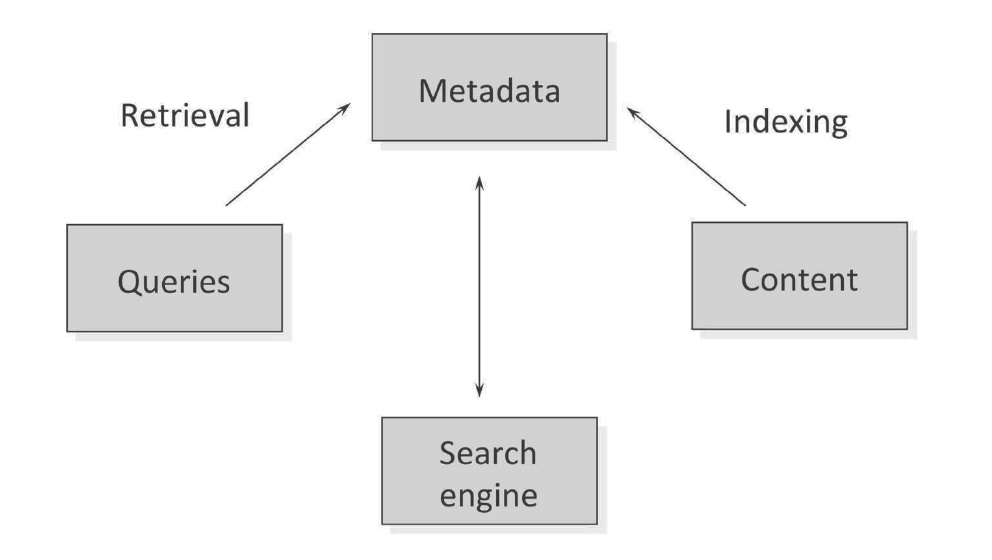
\includegraphics[width=\linewidth]{irprocess}
	\caption{Basis of Information Retrieval (IR) process.}
	\label{fig:1}
\end{figure}

The intelligent portal is built on top of the Figure \ref{fig:1}, which depicts a high-level perspective of the IR process. A person's information requirements to retrieve the \textit{content} is the primary focus of the IR process. The first step is to ask the IR system a \textit{query}. Metadata is used by \textit{search-engine} to match a user's query with relevant material. In IR, there are two types of thinking. Metadata are assigned to content objects during the \textit{indexing} process; \textit{retrieval} occurs when a user does a search and receives the results of that query \citep{prob2}.

\section{Intelligent Chatbot}

In the last decade, individuals have turned more and more to chatbot technology for help with things like social and emotional support and finding information \citep{chat1}. Chatbots, also known as conversational interfaces, allow computers to engage with humans in a more natural way \citep{chat2}. Conversation agents, dialogue assistants, and intelligent virtual assistants are all names for chatbots. Although chatbots have gained popularity among academics, developers, and end users, little is known about how well they can assist those living with dementia (which includes Alzheimer's disease and associated dementias) or those who care for them. This research also fills the knowledge gap by conducting a comprehensive assessment on available chatbots with a dementia emphasis.

A new research found that although AI chatbots show promise in helping dementia patients and aiding carers, the technology still has a long way to go before it is genuinely effective and dependable \citep{chat3}. Six chatbots were included in the study, and the researchers used an evidence-based evaluation technique to evaluate the quality and breadth of each. The chatbots were evaluated based on how well they might aid those with dementia and their caretakers. Five of the bots were voice-activated Alexa Skills, while the sixth was a smartphone app that only communicated through text. Some applications were made to assist patients remember things, while others were made to teach others about dementia. The applications were graded on how well they performed, how useful they were, how they made people feel, how happy they made them, how satisfied they made them, and how ethically they behaved.

\section{Aim and Objectives}
Long-term carers of persons with dementia may find it difficult, to access essential information and support. There are no such intelligent portal which might be helpful for the better care support in the field of dementia. When categorising the technologies, it is needed to take into account who would be the primary customers and benefactors of each one, where they would be located in the care environment, and how advanced their dementia was. The aim of this research is to develop a novel data driven intelligent information and resource portal based on the specific needs of the caregiver to any given situation. And, the objective refers to application of intelligent information retrieval methods coupled with current real-world data on resources and services to direct the right information for each contextualized query. The resource portal should be more intelligent that can reflect AI knowledge. An intelligent chatbot can be functioned adequately to help user with their queries, since they were not too difficult to master for the average user. 

The aim of this dissertation is to develop an intelligent resource portal for caregivers to help with people who have dementia. The associated objectives are:
\begin{enumerate}[label=\arabic*)]
	\item To study the relevant literature review and related works.
	\item To collect and gather required informations and resources regarding the dementia people. 
	\item To design and implement an intelligent portal with essential features.
	\item To test the developed system with collected data and helpful information.
\end{enumerate}

The purpose of this study is to accommodate for the distinct physical and cognitive deficiencies of dementia patients while also reducing carers stress with the help of artificial intelligence. In the health care and medical fields, the idea of information portals is not new, and there are a number of portals that give access to information and services on a wide range of health-related topics \citep{am1}. To suit the demands of individual users, more and more portals are being created to offer an intelligent interaction among consumers and relevant information resources. There are a slew of cutting-edge health care portals accessible right now. WebMD and HealthCentral.com are two healthcare websites with searchable healthcare information. Access to the portal may be customised based on the user's preferences, requirement, level of security, and accessible authorisation \citep{am2}. The research will help to build a intelligent information portal for the caregiving of people who have dementia.

\goodbreak

\section{Structure of Dissertation}
The rest of the dissertation structure will emphasize on:

\begin{enumerate}[label=$\ast$]
	\item Literature review - This section will highlight all the literature work related to the topic. It will also focus on the chatbot technology on health. Natural Language Processing and IR methods will also be reviewed here.
	\item Analysis - In this part, it will go through the proposed solution and software development process. All necessary software and hardware components, both internal and external, are listed. The project timeline and expected completion dates for each milestone will be shown graphically using a Gantt chart.
	\item Design - In this part, it will showcase web portal's overarching design, complete with user interface (UI) designs and storyboards that lay out the GUI in great detail. A visual representation of the technological architecture, such an activity diagram, will be created and presented. It will explain the interplay between all of the parts. Database structure and connections will be presented.
	\item Implementation and Testing - This section will detail the steps used in creating the solution's implementation. Unit testing and relevant test cases will be used to validate the chatbot and other features after development is complete. If any problems are found, they will be addressed to achieve the highest possible standard.
	\item Evaluation - The finished product is going to be assessed in order to establish both its level of quality and its overall worth. It will go into depth on the process that was used to build the entire project. When thinking back on the experience as a whole, it's important to point out both the aspects of the project that went particularly well and the ones that may need some tweaking for the future.
\end{enumerate}

\goodbreak
   


\def\baselinestretch{1.66}
\medskip


%%% ----------------------------------------------------------------------
